\documentclass[12pt,letterpaper]{beamer}
\usetheme{Copenhagen}
\usecolortheme{seahorse}
\setbeamertemplate{section in toc}{\inserttocsection}

\usepackage[utf8]{inputenc}
\usepackage{amsmath}
\usepackage{amsfonts}
\usepackage{amssymb}
\usepackage{graphicx}
\graphicspath{ {./images/} }
\usepackage{hyperref}
\hypersetup{
    colorlinks=true,
    linkcolor=blue,
    filecolor=magenta,      
    urlcolor=cyan,
    pdftitle={Overleaf Example},
    pdfpagemode=FullScreen,
}
\title[Robotics I]
{ENGR 3421: ROBOTICS I}
\subtitle{Into the Autonomous Ground Vehicle}

\author[Zhang, Lin]
{Dr. Lin Zhang}
\institute[UCA] % (optional)
{
  Department of Physics and Astronomy\\
  University of Central Arkansas
}
\date[Robotics1 2021] % (optional)
{August 19, 2021}
\logo{
\includegraphics[height=1cm]{uca-bear-logo.png}}


%End of title page configuration block
%------------------------------------------------------------

%------------------------------------------------------------
%The next block of commands puts the table of contents at the beginning of each section and highlights the current section:

\AtBeginSection[]
{
  \begin{frame}
    \frametitle{Outline}
    \tableofcontents[currentsection]
  \end{frame}
}
%------------------------------------------------------------

\begin{document}

%The next statement creates the title page.
\frame{\titlepage}
\begin{frame}
    \begin{alertblock}{Safe First!}
        Don't forget eyes and hands protection!
    \end{alertblock}
    Go over the \href{https://github.com/linzhangUCA/robotics1-2021/blob/main/syllabus_fall2021.pdf}{syllabus} for policies and contents.
\end{frame}

%---------------------------------------------------------
%This block of code is for the table of contents after
%the title page
\begin{frame}
\frametitle{Outline}
\tableofcontents
\end{frame}
%---------------------------------------------------------


\section{What is a Robot}

\begin{frame}{In Popular Culture}
    A robot is a machine resembling a human being and able to replicate certain human movements and functions automatically.
    \begin{figure}
        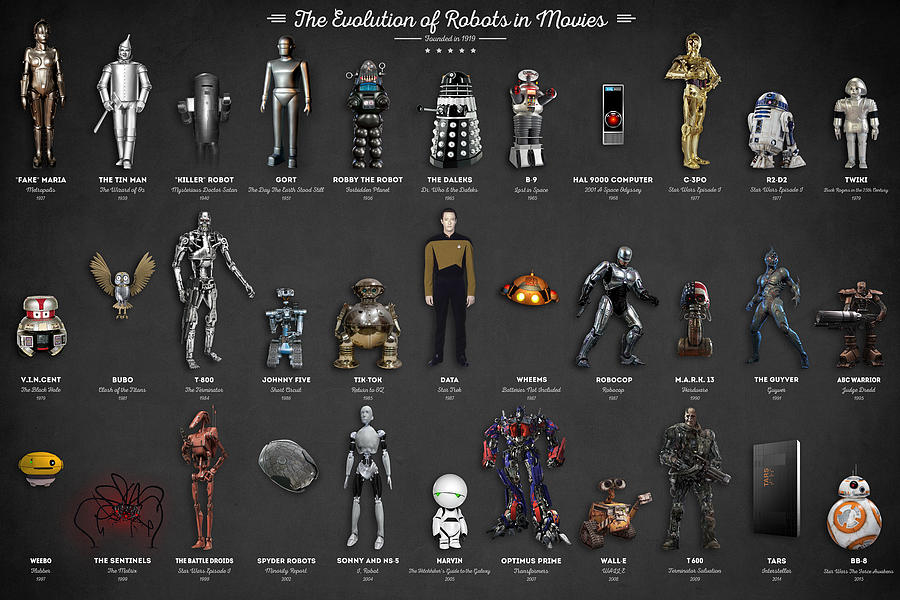
\includegraphics{evolution-of-robots-in-movies.jpeg}
        \caption{Robots!!}
    \end{figure}
\end{frame}

\begin{frame}{In Real World}
    Robots may be constructed to evoke human form, but most robots are task-performing machines, designed with an emphasis on stark functionality, rather than expressive aesthetics. 
    
    \href{https://youtu.be/k1GLwS7CVZs}{Car factory robots} \\
    \href{https://youtu.be/X2pOYXyx6xE}{Vaccum clean robots } \\
    \href{https://youtu.be/IMPbKVb8y8s}{Warehouse robots} \\
    \href{https://youtu.be/8cJ54TWGzMU}{Agricultural robots} and \href{https://youtu.be/hGyLjO7KWeU}{DJI solutions} \\
    \href{https://youtu.be/44KvHwRHb3A}{Lightshow drones} \\
    \href{https://www.amazon.com/dp/B0107H5FJ6/}{Toys}
    
\end{frame}

\begin{frame}{In Scientific/Engineering Research}
    A robot is a machine—especially one programmable by a computer—capable of carrying out a complex series of actions automatically. 
    
    \href{https://youtu.be/tF4DML7FIWk}{Humanoid} \\
    \href{https://youtu.be/9j2a1oAHDL8}{Quadrupedal robot} \\
    \href{https://youtu.be/-q8D7BcLjac}{Spherical robot} \\
    \href{https://youtu.be/hUE8o056Cpc}{Flapping robot} \\
    \href{https://youtu.be/Hebpmadjqn8}{Quadrotor $/$ Drone} \\
    \href{https://youtu.be/4WOOwesIkss}{Underwater robot} \\
    \href{https://youtu.be/qevIIQHrJZg}{Soft robot} \\
    \href{https://youtu.be/5qqsMjy8Rx0}{Extra-terrestrial rover} \\
    \href{https://youtu.be/m-LP4qpOLl0}{You name it...}

\end{frame}

\begin{frame}{Autonomous Ground Vehicle (AGV)}
    A.k.a. automated guided vehicle, mobile robot, unmanned ground vehicle (UGV). 

    \href{https://youtu.be/fmVWLr0X1Sk}{Self-driving cars} \\ 
    \href{https://youtu.be/dagjQW_jgtE}{Delivery robots} \\
    \href{https://youtu.be/IMPbKVb8y8s}{Warehouse robots} 

\end{frame}

\begin{frame}{}
    \href{https://youtu.be/EezdinoG4mk}{Build it, Break it, Fix it}
    
\end{frame}

%----
\section{Our Robot}

\begin{frame}
\frametitle{Our Robot}

\begin{columns}

\column{0.5\textwidth}
% Figure here
\begin{figure}
    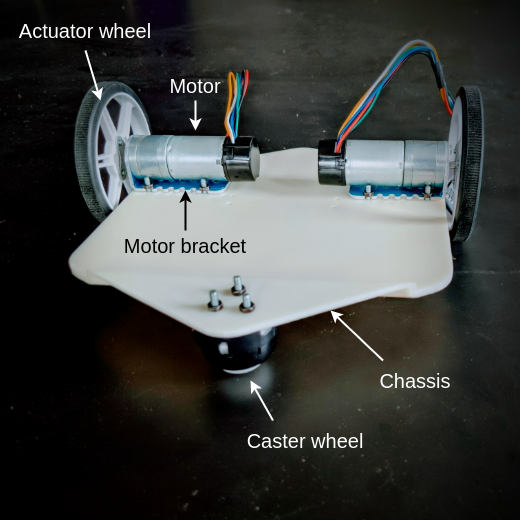
\includegraphics[width=0.8\textwidth]{3421bot}
\end{figure}

\column{0.5\textwidth}
Most parts (all except the chassis) are purchased from \href{https://www.pololu.com/}{Pololu}
{\scriptsize 
\begin{itemize}
    \item Chassis (\href{https://github.com/linzhangUCA/robotics1-2021/blob/main/0819/chassis_v3.stl}{3D model})
    \item \href{https://www.pololu.com/product/2691}{Caster wheel} (Pololu \#: 2691) 
    \item \href{https://www.pololu.com/product/2676}{Motor brackets} (Pololu \#: 2676)
    \item \href{https://www.pololu.com/product/4805}{Motor} (Pololu \#: 4805)
    \item \href{https://www.pololu.com/product/3690}{Actuator wheel} (Pololu \#: 3690)
\end{itemize}

}
\begin{block}
\footnotesize 3D printer @ CCCS 112
\end{block}

\end{columns}

\end{frame}
%---------------------------------------------------------



\section{Github Classroom}
\begin{frame}{Github}
    \href{https://github.com}{GitHub} is a website and cloud-based service that helps developers store and manage their code, as well as track and control changes to their code. 
\end{frame}

\begin{frame}{Github Classroom}
\begin{itemize}
    \item \href{https://classroom.github.com}{GitHub Classroom} automates repository creation and access control, making it easy to distribute starter code and collect assignments on GitHub.
    \item This is the place you'll complete most (if not all) of your assignments.
\end{itemize}


\begin{alertblock}{Note}
{\footnotesize 
\begin{itemize}
        \item Access Github Classroom: \href{https://classroom.github.com}{https://classroom.github.com}
        \item Check your email for my invitation.
    \end{itemize}
}
\end{alertblock}   

\end{frame}

\end{document}
